%; whizzy chapter
% -initex iniptex -latex platex -format platex -bibtex jbibtex -fmt fmt
% 以上 whizzytex を使用する場合の設定。

%     Tokyo Debian Meeting resources
%     Copyright (C) 2006 Junichi Uekawa

%     This program is free software; you can redistribute it and/or modify
%     it under the terms of the GNU General Public License as published by
%     the Free Software Foundation; either version 2 of the License, or
%     (at your option) any later version.

%     This program is distributed in the hope that it will be useful,
%     but WITHOUT ANY WARRANTY; without even the implied warranty of
%     MERCHANTABILITY or FITNESS FOR A PARTICULAR PURPOSE.  See the
%     GNU General Public License for more details.

%     You should have received a copy of the GNU General Public License
%     along with this program; if not, write to the Free Software
%     Foundation, Inc., 51 Franklin St, Fifth Floor, Boston, MA  02110-1301 USA

%   Pdf作成手順
% dvipdfmx debianmeetingresume200510-kansai.dvi

%%ここからヘッダ開始。

\documentclass[mingoth,a4paper]{jsarticle}
\usepackage[dvipdfmx]{graphicx}
\usepackage{fancybox}
\usepackage{longtable}
\usepackage{ascmac}	% 囲み (screen,itembox)
\usepackage{fancyvrb}   % 囲み Verbatim のために必要
\usepackage[dvipdfmx]{hyperref}
\usepackage{url}

%http://www.naney.org/diki/dk/hyperref.html
%日本語EUC系環境の時
\AtBeginDvi{\special{pdf:tounicode EUC-UCS2}}
%シフトJIS系環境の時
%\AtBeginDvi{\special{pdf:tounicode 90ms-RKSJ-UCS2}}

%% spacing の設定をする。外枠を減らす。
\setlength\headheight{0mm}
\setlength\topmargin{-20mm}
\setlength\headsep{0mm}
\setlength\topskip{3mm}
\setlength\maxdepth{4pt}
\setlength\columnsep{6mm}
\setlength\textheight{252mm}
\setlength\topmargin{-5mm}
\setlength\textwidth{170mm}
\setlength\oddsidemargin{-5mm}
\setlength\evensidemargin{-5mm}

% commandline環境を定義。画面入出力についてはcommandline環境
% で表記する
\newenvironment{commandline}%
{\VerbatimEnvironment
  \begin{Sbox}\begin{minipage}{15cm}\begin{fontsize}{7.3}{7.3} \begin{BVerbatim}}%
{\end{BVerbatim}\end{fontsize}\end{minipage}\end{Sbox}
  \setlength{\fboxsep}{8pt}\fbox{\TheSbox}}

%%% start of santaku
\makeatletter
\newwrite\tf@jqz
\immediate\openout\tf@jqz\jobname.jqz\relax
\makeatother
\newcounter{santakucounter}
\newcommand{\santaku}[5]{%
\addtocounter{santakucounter}{1}

\addtocontents{jqz}{\arabic{santakucounter}. #5\\}
\nopagebreak 問題\arabic{santakucounter}. 
#1\\
\nopagebreak□ A #2\\
\nopagebreak□ B #3\\
\nopagebreak□ C #4
\pagebreak[1]
\hspace{1cm}
\\

}
%%% end of santaku


\newcommand{\emptyspace}{(\underline{\hspace{1cm}})}



\newcommand{\subsubsubsection}[1]{%
\vspace{1zw}{\bf #1}\\}


% sectionをセンタリングする
\makeatletter
  \renewcommand{\section}{\@startsection{section}{1}{\z@}%
    {\Cvs \@plus.5\Cdp \@minus.2\Cdp}% 前アキ
    {.5\Cvs \@plus.3\Cdp}% 後アキ
    {\normalfont\Large\headfont\raggedright\centering}} % style
\makeatother

% section の代わりの環境
\newcommand{\dancersection}[2]{%
\newpage
東京エリアDebian勉強会 2005
\hrule
\vspace{0.5mm}
\hrule
\hfill{}
\includegraphics[width=3cm]{image200502/openlogo-nd.eps}\\
\vspace{-4cm}
\begin{center}
  \section{#1}
\end{center}
\hfill{}#2\hspace{3cm}\space\\
\hrule
\hrule
\vspace{1cm}
}

\begin{document}


\begin{titlepage}

% 毎月変更する部分, 本文の末尾も修正することをわすれずに
\title{
2005年 東京エリア Debian 勉強会、関西出張版\\事前資料}
\date{2005年10月29日}
\author{Debian勉強会会場係 上川 純一\thanks{Debian Project Official Developer}} 
\maketitle
\thispagestyle{empty}

\end{titlepage}

\newpage
\tableofcontents

\dancersection{Introduction To Debian 勉強会}{上川 純一}

今月のDebian勉強会へようこそ。
これからDebianのあやしい世界に入るという方も、すでにどっぷりとつかってい
るという方も、月に一回Debianについて語りませんか?

目的として下記の二つを考えています。

\begin{itemize}
 \item メールではよみとれない、もしくはよみとってられないような情報を情
       報共有する場をつくる
 \item まとまっていないDebianを利用する際の情報をまとめて、ある程度の塊と
       して出してみる
\end{itemize}

また、東京にはLinuxの勉強会はたくさんありますので、Debianに限定した勉強
会にします。Linuxの基本的な利用方法などが知りたい方は、他でがんばってくださ
い。
Debianの勉強会ということで究極的には参加者全員がDebian Packageを
がりがりと作りながらスーパーハッカーになれるような姿を妄想しています。

Debianをこれからどうするという能動的な展開への土台としての空間を提供し、
情報の共有をしたい、というのが目的です。
次回は違うこと言ってるかもしれませんが、御容赦を。

\subsection{講師紹介}

\begin{itemize}
 \item{やまね} reportbug の使い手です。
 \item{上川 純一} dpkg-dev-el, debian-el の使い手です。
\end{itemize}

%%% trivia quiz
\dancersection{Debian Weekly News trivia quiz}{上川 純一}

ところで、Debian Weekly News (DWN)は読んでいますか?
Debian 界隈でおきていることについて書いているDebian Weekly News.
毎回読んでいるといろいろと分かって来ますが、一人で読んでいても、解説が少
ないので、
意味がわからないところもあるかも知れません。みんなでDWNを読んでみましょう。

漫然と読むだけではおもしろくないので、DWNの記事から出題した以下の質問にこたえてみてください。
後で内容は解説します。


\subsection{2005年37号}
2005年9月13日です。
%http://www.debian.org/News/weekly/2005/37/
 \santaku{バグトラッキングシステムの見栄えで最近かわったのは何か}
 {CSSを利用するようになった}{DHTMLになった}{XHTMLになった}{A}
 \santaku{Debian UKで問題になったのは何か}{メンバーが活動的でないこと}
 {UKの経済状況がよろしくないこと}{商用利用をしようとした場
 合のDebianという名前の商標の利用の許可をする基準が不明確だったこと}{C}
 \santaku{ソフトウェアを計測する、という論文で発表されたのは何か}{Debian
 sarge には2億3000万行のソースコードが含まれている}{Debian sargeの品質を
 計測した}{Debian sargeの利用しやすさを計測した}{A}
 \santaku{Joey Hess は testing に対して security 対応をすることを発表した。
 それに利用しているサーバはどれか}
 {secure-testing.debian.net}{security.debian.org}{security.debuan.org}{A}
 \santaku{/usr/docをいまだにつかっているパッケージ数はどれくらいか}{100}{200}{500}{C}%C
 \santaku{planet.debian.orgをメーリングリスト経由で配布しようという意見
 に対して出た反論は}{blogの内容は機密事項なので、メーリングリストで配布
 してほしくない}{メーリングリストとして配布するとサーバの負荷が高くなる}{blogの内容を永続的にメーリングリストのアーカイ
 ブとして保存されたくない}{C}%C
 \santaku{/usr/share/doc/パッケージ名/examples/ にあるファイルに実行権限
 をつけることについてはどうするべきか}{サンプルは実行できるものは
 実行権限をつけるべき}{サンプルなんてかざりなので実行しなくてよい}
 {/usr/share以下について実行権限をつけるのはこのましくなく、実行ファイルはbinにおくべきだ。}{C}
 \santaku{sponsors.debian.netが提供するサービスは何か}{金銭的寄付をつの
 るフィッシングサイト}{広告を配信し、広告収入をDebianプロジェクトの発展
 のために利用するサイト}{まだメンテナ
 になっていない人が管理しているパッケージについてスポンサーが必要な状況
 をトラッキングするシステム}{C}
 \santaku{1.0beta3のようなベータ版のバージョン番号が1.0のような最終版の
 バージョン番号より低い、とdpkgが判定してしまう。この状況に関してメンテ
 ナはどう対応するべきか}
 {優先度の低い チルダ記号 \~{ }を利用して、 1.0\~{
 }beta3のような名前にする。
ただまだアーカイブシステムが対応していないので、今後の改善が必要。}{あき
 らめる}{ベータ版はパッケージ化しない}{A}
 \santaku{ソースのみのパッケージのアップロードを可能にするという提案についての反論は
 何か}{バイナリが必要でなくなると、メンテナがテストをしなくなるのではな
 いだろうか、という懸念がある}{ソースのみだとパッケージインフラが破綻す
 る}{katieを改変するのが面倒}{A}
 \santaku{BTSに任意のタグを追加できる機能が追加された、なんという機能か}
 {tagtag}{たぐるんです}{usertag}{C}

\subsection{2005年38号}
2005年9月20日です。
%http://www.debian.org/News/weekly/2005/38
 \santaku{David Moreno Garzaがwnppにてcloseしたバグレポートの数は}{729の
 バグレポート}{100のバグレポート}{123のバグレポート}{A}%A
 \santaku{International Conference on Open Source Systemsに投稿された論
 文の中で説明されていた結果は}{開発者は短期間でどんどん入れ替わる}{メン
 テナは実は幻想で、そんな人は存在しない}{長いあいだアクティブに活動し、パッケー
 ジの数も多くメンテナンスする}{C} % c
 \santaku{Frank Lichtenheldが発表したのは、non-freeなドキュメントを削除
 する処理を開始するということだった。状況をトラッキングするために彼が利
 用したインフラは。}{BTSののusertags機能で
 debian-release@lists.debian.orgユーザのタグとして管理}{
 Wikiページ}{CVS管理のテキストファイル}{A}% A
 \santaku{Software freedom day 05でDebian-womenが行って、
 結果として良かったので今後も継続することになったのは}{debian-women-new
 IRCチャンネルがよい結果をもたらしたので、今後はdebian-womenチャンネルに
 新人を歓迎する時間帯というのをもうける}{CDをたくさん焼いたら人気だった}
 {KatieやBTSなどをインストールしてユーザがいじれるように提供したら人気だったので、今後もやる}{A}
 \santaku{init.dスクリプトは現在直列に実行されているが、今後
 、並列実行を実装する際に便利だろうと思われる
 LSB規格の仕様は}{なんとなく並列に実行しても壊れないようにする仕様}{
 気持の中だけでは並列な年頃}{initスクリプトの中で依存関係を記述できる仕様}{C}
 \santaku{新しいバージョンのパッケージにて問題が解決した場合の、バグレポー
 トをクローズする方法でないのは何か}{changelogでバグ番号を記述し
 アップロードする}
 {バージョンヘッダを付けて、リクエストを -done アドレスに投げる}{btsclose
 コマンドを利用する}{C} %c
 \santaku{Marc Brockschmidtが説明した、新規メンテナプロセスのFront Desk
 の変更とは}{
今後はより厳しい思想チェックを行う}{Debianに
 コントリビュートしていることが要件になり、何もしていない場合は、応募が
 取り消される}{年齢制限を設けます}{B}
 \santaku{security.debian.orgで問題になったのは何か}{セキュリティーアッ
 プデートが遅い}{セキュリティーアップデートが嘘だった}{xfree86のセキュリ
 ティーアップデートがあまりにも高いネットワーク負荷を発生させてしまい、
 security.debian.orgがサーバとして機能しなくなってしまった。}{C}
\subsection{2005年39号}
2005年9月27日です。
%http://www.debian.org/News/weekly/2005/39/
 \santaku{Ben HutchingがDebconfについて報告したのは}{もう終ってしまった
 事は忘れる}{忘れ物がありました}{DVDが入手可能に
 なった}{C}
 \santaku{wiki.debian.orgへの移行で特に手動の労力が必要だったのはどこか}
 {すでにwiki.debian.netからwiki.debian.orgに移行してしまっているページが
 いくつかあったのでそれに対しての手動の対処}{kwikiからmoinmoinへデータ形
 式の変更}{ドメイン名の登録}{A}%Aのつもり
 \santaku{initの時点では/がread-onlyでマウントされているが、その時点でデー
 タを保存するのにはどうしたらよいか。}{メモリファイルシステムを/runにマ
 ウントする}{/mnt以下にメモリファイルシステムをマウントする}{/をrwにマウ
 ントしなおす}{A}
 \santaku{グラフィックライブラリ GLU の実装がDebian内で複数ある理由はな
 ぜか}
 {一部のコードが一部のハー
 ドウェアでしか動かないという状況が続いているから}
 {複数のパッケージをメンテナンスしているほうがかっこいいから}{メンテナの
 仲が悪いから}{A}
 \santaku{Jeroen van Wolffelaarが提案したのは}{libc5を消す}{libc6を消す}
 {libc6.1を消す}{A}%A
 \santaku{piupartsであきらかになる問題は}{purgeする際に、essentialでは
 ないパッケージに依存して、動作しないパッケージ}{インストールしても動かないパッ
 ケージ}{使ってみて使いにくいパッケージ}{A}

\subsection{2005年40号}
2005年10月4日です。
%http://www.debian.org/News/weekly/2005/40/
 \santaku{DPLチームが今後検討する予定の問題について記録する媒体として選
 択したのは}{BTS}{IRC bot}{Wiki}{C}
 \santaku{tetex 3.0はどういう状況になっているか}{今後も入る見通しがない}
 {うごかなくて困っている}{experimentalにアッ
 プロードされ、ライブラリのフリーズが完了したらunstableに入る}{C}
 \santaku{Debian で配布するIA64アーキテクチャ向けのカーネルについて
 Dann FrazierがSMPじゃないカーネルのサポートを削除しようとした、何故か}
 {SMPじゃないといやだから}{時代はSMPです}{IA64で、SMPでないシステムがほ
 とんどなく、あまりテストされていない}{C}
% Chris LameterはSMPじゃないシス
% テムも仮想化環境用などで必要だろうと説明しているが、Debianがそれをすべ
% きかというと違うだろう。
 \santaku{Wolfgang Borgert によると
planet.debian.orgと、メーリングリストの利用方法の違いは}
{メーリングリストは古い技術なので今後はつかわなくなる}{blogはフレームされないで意見を述べることのできるメディアだが、議論す
るのはメーリングリストでして欲しい}{planet.debian.orgは安定していないの
で使わないで欲しい}{B}
 \santaku{pbuttonsdは/dev/input/eventXXを利用しているが、どういう問題が
 あったか}{makedevが、最大32あるうちの4個しかデバイスファイルをつくっていなかっ
 たので、/devを静的に管理しているユーザは一部の機能を利用できていなかっ
 た。}
 {USB接続ではうまく認識できなかった}{電源ボタンがおされたらアプリケーショ
 ンがハングした。}{A}

\subsection{2005年41号}
2005年10月11日です。
%http://www.debian.org/News/weekly/2005/41/
 \santaku{Debian securityで改善したのは}{バックエンドとフロントエンドの
 サーバを分割し、負荷に強い構成に変更した}{特定のユーザが負荷をかけられ
 ないようにスロットリングした}{セキュリティーパッチをリリースしないこと
 でサーバに負荷がかからないようにした}{A}
 \santaku{Carlos Parra Camargoが報告したのは何か}{Wikiが悪意をもったユー
 ザにより書き換えられていたので前のバージョンを復活させた}{Wikiがおもし
 ろくないので改善しよう}{Wikiサーバがダウンしている}{A}
 \santaku{mozilla 1.7.8に対してのセキュリティーアップデートはどういう形
 でリリースされたか}{1.7.10にバージョン1.7.8という名前をつけてリリースし
 た}{セキュリティーパッチをバックポートした}{セキュリティーホールのある
 機能を全てdisableにした}{A}
 \santaku{複数のchrootで同じユーザ情報を利用するのに利用できる方法でない
 のは}{FUSEのshadow etc}{LDAP}{rm /etc/passwd}{C}
 \santaku{ソースコードにローカルに適用したパッチをパッケージの
 アップグレード後も維持するためにはどうしたら一番楽か}
{自分でがんばる}{apt-srcを利用する}{パッチはあてない}{B}
 \santaku{Jurij Smakovがリリースした文書は何か}{Debian Users Handlebook:
 Debianユーザをどうあつかえばよいのか、が書いてある}{Debian Developers
 Handlebook: Debian Developerをどう扱えば良いか、が書いてある。
}{Debian Linux Kernel
 Handbook: Debianでカーネルがどうビルドされているのか、が書いてある}{C}
%http://kernel-handbook.alioth.debian.org/

\subsection{2005年42号}

% http://www.debian.org/News/weekly/2005/42/
% 10月18日

\santaku{Eliveって何?}
{電子的に生きること}
{enlightenmentベースのLiveCD}
{Eliseの新しいバージョン}
{B}

\santaku{m68kについてSteve Langasek が発表したのは}
{m68kを自分もつかいたい}
{m68kがDebianの移植版の中で一番素晴らしい}
{testingに入る条件として、m68kは無視することにした}
{C}

\santaku{etch向けのdebian-installerの状況はどうか}
{もう全アーキテクチャについてインストールできることは確認した}
{もうすでに完全に動いている}
{まだ一部のアーキテクチャではビルドできない}
{C}
% \url{http://people.debian.org/~igloo/status.php?packages=debian-installer}

\santaku{gnome1のパッケージがビルドできなくなったのはなぜか}
{古いから}
{libpng10が削除されたから}
{gnome2の時代がやっときたから}
{B}

\santaku{ Edd Dumbillが、sargeをインストールする際に、debian-installerを利用しているときに
ハードウェアの問題にあたったときに利用するように提案したのは}
{knoppixでハードウェア認識}
{ハードウェアを買い替える}
{Debianを使う事をあきらめる}
{A}

\santaku{Oldenburg のミーティングの結果として、
Debian security updateでBranden Robinsonが報告したのは}
{security.debian.orgのバックエンドサーバが冗長構成になった}
{security.debian.org サーバがDNSのラウンドロビンで3台存在している構成がとれるようになった}
{security.debian.orgがフィッシングサイトになった}
{B}

\santaku{ソフトウェアに含まれている画像のライセンスにCreative Commons
BY-SAライセンスを利用したものはGPLのパッケージに含める事ができるか}
{やめたほうがよい}
{可能}
{MJ Rayによると、不可能なため、そのような場合はMITライセンスを利用したほうがよい}
{C}

\santaku{Camm McGuireがlibbfdにリンクするのにはどうしたらよいのだ、と質
問したときのDaniel Jacobwitzの回答は}
{libbfdは安定しているのでいくらでもリンクしてくれ}
{よくバイナリレベルの互換性は破壊されるので、binutils-devにあるlibbfd.a
をつかってくれ}
{一般人はlibbfdは使うな}
{B}



\subsection{2005年43号}

% http://www.debian.org/News/weekly/2005/43/
% 10月25日
\santaku{Joerg JaspertがNEWのパッケージをREJECTする理由で多いと指摘したのは}
{読めないドキュメントが多い}
{おもしろくないパッケージが多い}
{debian/copyrightが不正確なものが多い}
{C}

\santaku{Steve Langasek が宣言したetchのリリーススケジュールによると、
etchがリリースされるのは}
{2005年12月}
{2006年6月}
{2006年12月}
{C}

\santaku{今月、Christian Perrierが宣言したかなり完成している、とコメント
していたdebian-installerの機能は何か}
{sidをインストールするインストーラ}
{etch向けのテキストモードのインストーラ}
{GTKを利用したグラフィカルインストーラ}
{C}

\santaku{ypbindなどが動的にポートを確保する場合、その後に起動する
サーバとポート番号がかぶる場合があるそれを回避する方法は}
{portreserve}
{祈る}
{nisなんて使わない}
{A}

\santaku{/etc/hostsに書いてある127.0.0.1のホスト名は現在のsidでは何にな
るか}
{ホスト名}
{localhost.localdomain}
{localhost}
{B}

\santaku{slang用のモジュールパッケージ名は今後'slang-モジュール名'という
形になりそうだが、従来はどういう名前だったか}
{slモジュール名}
{モジュール名-slang}
{モジュール名}
{A}

\santaku{pbuilderの開発体制にどういう変化があったか}
{名前が変わりました}
{チームメンテナンス制をとるために、aliothに移動した}
{おもしろくなくなってきたのでもうやめます}
{B}

\santaku{Daniel Ruosoが提案したDebianの移植版は}
{uclibc移植版}
{minix 3.0 移植版}
{z80移植版}
{A}

\santaku{curlについてopenssl版とgnutls版の両方を提供するようになった、その
理由は}
{GPLのプログラムがopensslとリンクしなくてすむように}
{二種類あったほうが楽しいから}
{GNUのほうがopensslより凄いから}
{A}

\dancersection{最近のDebian関連のミーティング報告}{上川 純一}

\subsection{東京エリアDebian勉強会9回目報告}


前回開催した第9回目の勉強会の報告をします。

当日のタイムテーブルは下記でした
\begin{itemize}
 \item 18:10- quiz
 \item 18:30- こたえあわせ
 \item 19:00- 休憩
 \item 19:10- たるさん
 \item 20:10- 上川
 \item 21:00- 宴会
\end{itemize}

10月の第9回東京エリアdebian勉強会報告。
今回はdebbugsについての熱い話しを展開しました。
今回の参加人数は登録者が11名くらいで、実際に参加したのが9名くらいでした。

DWN quizに関しては、今回は小林さんが1問不正解で最高点数でした。

たるいしさんがapt-listbugsについて説明しました。
昨年のAsia Debian Mini Confで発表した内容を説明して、
実はそのころのTODOは進捗していない、ということを説明していました。
osdn.debian.or.jp でミラーしているのですが、rsync もとはもともと master.debian.orgだったが、
同期できていないというバグ報告があって気づいて、 merkel.debian.org に切替えたという話しがでていました。
資料にあるグラフは2003年9月から2004年10月で今は一年たっているので、おそ
らく7000IPアドレスからの利用があるのだろう、と予想していました。
また、中国で発表したときに、使ってみたら、バグの情報を取得するのに何分もかかり、
ミラーサーバ必要だ、という話になった、がいまだになにもできていないとか、
RSSViewerを使えば、自分のマシンに今入っているパッケージのセキュリティー
関連のバグだけを見る、ということができる。
実は便利かもしれない、とか。
メンテナンスにあきてきたのでどうせならかきなおしたいなぁという宣言もでていました。

上川が、Anthony TownsがFinlandのdebconfで発表していた内容と、
その後にその発表に触発されて実装されたDebbugsの新機能について話しました。
おそらくDebbugsの仕様について日本語で記述した資料はこれが初めてなのではないでしょうか。
新しい機能がいろいろと実装されており、apt-listbugsでも利用できそうな情報もあるので、
たるいしさんの今後のハックに期待です。


\dancersection{``claim'' makes Debian better}
{やまね}
\label{sec:yamane}
%%yamaneさんの記事はここから

\subsection{本日の目的}

Debian BTSについて理解を深める

\begin{itemize}
\item BTSって何さ?
\item どういうときにするの?
\item 何がいいの?
\item 実際どうすればいいの?
\end{itemize}

そして立派なクレーマーとして認められる!

\subsection{Debian Bug Tracking System}

Debian独自のバグ追跡システム。
システムとしてはdebbugsという独自のものを利用

\subsubsection*{特徴}

\begin{itemize}
\item Webから閲覧可能(まぁ、最近のは皆そうですね)
\item やり取りは基本的に全てオープン
\item メールベースで作業が進む(ここは珍しいかも)
\item かなり使い込まれてます。30万件近くが登録済み。\\
redhatのbugzillaはこの半分ぐらいの件数
\end{itemize}

\begin{figure}[htbp]
\begin{center}
\includegraphics{image200508/bts.eps}
\end{center}
\caption{BTSのページ(http://www.debian.org/Bugs/)}
\label{bts-webpage}
\end{figure}

\subsubsection{どんなときにBTSを利用しますか?}

\begin{itemize}
\item パッケージングのバグに遭遇したとき
\item アップグレードしたらよくわからない現象が起こるようになってしまったとき
\item いつまで経ってもsecurity fixが提供されないとき
\item 気の利いた機能を実装したのでパッチを取り込んでもらいたいとき
\item 地味〜なL10Nな作業を取り込んでもらうとき
\item セキュリティホールの報告があったのでメンテナをせっつきたいとき
\end{itemize}

\subsubsection{擬似パッケージ (pseudo package)}

パッケージではないが、BTSで扱うためにパッケージとして扱うもの

\begin{itemize}
\item Webサイト
\item wnpp -- 作業が望まれるパッケージ(ITPも)
\item インストールシステム	などなど
\end{itemize}

\url{http://www.debian.org/Bugs/pseudo-packages.ja.html}参照

\subsubsection*{ここでのポイント}

あらゆる苦情・提案はBTSに集まる。誰も聞いていないところで文句を言うのではなくBTSすべし。

\subsection{BTS用ツール}

\subsubsection{reportbug/querybts}

\subsubsection*{reportbugコマンド}

簡単にバグレポート・レポートの検索が可能

\begin{itemize}
\item 対話的な操作が可能です。
\item レポートはメールで飛びます。ポーンと。
\item レポートはgnupgで署名も可能。まるでちゃんとした報告みたいに見えます。
\end{itemize}

\begin{figure}[htbp]
\begin{center}
\includegraphics{image200508/reportbug.eps}
\end{center}
\caption{reportbugの画面}
\label{reportbug}
\end{figure}

\subsubsection*{querybtsコマンド}

バグレポートの検索に特化しています。

\subsubsection{debbugs-el}

emacs ユーザは、 debbugs-el パッケージに含まれる debian-bug コマンドを使うこともできます。M-x debian-bug と入力すると、reportbug とよく似たやり方で、全ての必要事項を尋ねられます…らしい。(emacs使ってないので不明)

\subsection{「重要度」と「タグ」}

\subsubsection{Severity (重要度) レベル}

\url{http://www.debian.org/Bugs/Developer#severities}参照

\begin{itemize}
\item critical(致命的)

システム上の関係のないソフトウェア (またはシステム全体) を破壊する、重大なデータの欠落を引き起こす、または、そのパッケージをインストールしたシステム上でセキュリティホールが生じる場合。 

\item grave(重大)

問題のあるパッケージが使用できない、またはほとんど使用できない。またはデータの欠落を引き起こす、そのパッケージを使用するユーザのアカウントにアクセスを許してしまうセキュリティホールが生じる場合。 

\item serious(深刻)

Debian ポリシーに対して見すごせない違反がある (大まかに言うと、"must" や "required" の要件に違反している)、またはパッケージメンテナの意見としてそのパッケージがリリースに適していないと判断された場合。 

\item important(重要)

バグがパッケージの利用に大きく影響しており、対処しなければ誰にもまったく使用できない場合。 

\item normal(通常)

デフォルト値。通常のバグ。 

\item minor(軽度)

問題がパッケージの利用に影響しない、かつ修正はたいした事がないと思われる場合。 

\item wishlist(要望)

将来的な要望、主に設計上の理由により修正が非常に困難なバグ。
\end{itemize}

\subsubsection{タグ}

\url{http://www.debian.org/Bugs/Developer#tags}参照

\begin{itemize}
\item patch(パッチ)

バグ報告に、バグを修正するためのパッチや簡単な手順が含まれています。 パッチがあってもバグを適切に解決できない場合や別の問題を生じる場合は、 このタグは使うべきではありません。 

\item security(セキュリティ)

このバグはパッケージのセキュリティ問題を説明します。 ほとんどのセキュリティバグは、critical (致命的) や grave (重大) の severity (重要度) も設定すべきです。 

\item upstream(上流)

このバグは、パッケージの上流の部分に影響します。

\item d-i(インストーラ)

 このバグは、debian-installer に関するものです。 インストーラの開発に関係するけれども、インストーラの直接の 構成要素ではないパッケージに対するバグの場合、このタグを使ってください。 

\item L10n

このバグは、パッケージの地域化に関するものです。 

\item woody / sarge / sid / experimental

このバグは特に各ディストリビューション に加えられるものです。
\end{itemize}

\subsection{BTSの心得}

\begin{itemize}
\item 何よりも相手を尊重しよう
\item 事実を端的に述べよう
\begin{itemize}
\item 環境の記述は多すぎず少なすぎずを目指そう
\item バージョンやアーキテクチャぐらい書こう(面倒な人はツールを使いましょう)
\end{itemize}
\item broken English でもいいや、と開き直ろう
\item でも多少は体裁は整えておこう
\begin{itemize}
\item gnupg 使ってみるとか
\item 定型シグネチャ使っておくとか
\end{itemize}
\end{itemize}

\dancersection{Starting debconf translation}
{やまね}

\url{http://kmuto.jp/debian/po-trans/}に翻訳の状況が掲載されている。

\subsection{必要なもの}

\begin{itemize}
\item debconf-updatepo

poが最新のものかをチェック

\item msgfmt

文法があっているかをチェック
\end{itemize}

\subsection{手順}

\begin{enumerate}
\item po-debconfをインストール

\begin{commandline}
apt-get install po-debconf
\end{commandline}

\item 翻訳したいパッケージのソースをインストール

\begin{commandline}
apt-get source <packagename>
\end{commandline}

\item template.poをコピーして翻訳する

\begin{commandline}
cd <packagename>/debian/po
cp template.pot ja.po
\end{commandline}

\item 査読してもらう

debian-doc@debian.or.jpとかに投げる

\item BTSする

\begin{commandline}
reportbug -A 翻訳したファイル -g
ファイルを添付してGPG Signしてバグレポート送信
\end{commandline}

\end{enumerate}

%%ここまで

\dancersection{debbugs internal}{上川}
\label{sec:uekawa}
\subsection{はじめに}

この文書は Anthony Towns が フィンランドの debconf 5 で発表した内容を
日本にて展開するための資料です。
Anthony Townsの作成した英語の資料を省略して抜粋しています。
また、それ以降に変更した事項について追記しています。

Debian Bug Tracking System (BTS)は、ほぼDebianに特化したバグ報告の管理
のためのシステムです。
他のプロジェクトでも利用されていることもありますが、Debianでバグがパッケージベー
スで厳格に分類できることなどの特性が反映されているため、Debianプロジェク
トのワークフローで使いやすいように作られています。
\footnote{Debian のインフラと統合されており、changelogにバグ番号を記述してパッケー
ジをアップロードしたらバグが修正されたと記録されるようになっていたりします。}

規模としては、55000以上の現在アクティブなバグ報告、
231000のアーカイブされたバグ報告を現在保持していて、
毎週1000以上の新規のバグ報告が追加されています。
ウェブインタフェースは追加された報告をすぐに反映しており、
過去、ダウンタイムもほとんど発生していません。

Anthony Townsによると下記がバグトラッキングシステムの要件です。

\begin{itemize}
 \item インタフェース: 開発者がメールで操作できるようになっており、誰で
       もウェブで閲覧できるようになっている。
 \item パッケージベース: バグ報告をパッケージ別に高速に管理する必要があ
       る
 \item スケーラビリティー: 大量のバグ報告に対応できる必要がある
 \item 即時性: 現在のバグの状態をすぐに報告してくれる必要があり、バグの
       状態が変更されたらすぐに反映される必要がある
 \item 安定性: 継続して動作する必要がある。新規の機能がどんどん追加さ
       れたとしても。
 \item 公開: 議論の内容にDebianコミュニティー全体として参加できるように、
       永続的な公開記録として保存される必要がある。
\end{itemize}

\subsection{データ形式}

バグデータベースのスプールの形式は下記です。
リレーショナルデータベースなどは利用していません、
スプールディレクトリ以下にほとんどのデータが格納されています。

各バグについて、ファイルはそれぞれ
4個あります。
サマリーファイルはメタデータを保存します。
ログファイルは、そのバグに対して流れたメールを全て保存します。

statusファイルは互換性のためだけに存在しています。
reportファイルは、最初のバグ報告のメールで、バグが close されるときに送
信されるものです。

\begin{itemize}
 \item /org/bugs.debian.org/spool
       \begin{itemize}
	\item incoming/
	      \begin{itemize}
	       \item T.*
	       \item S[BMQFDU RC] *.*
	       \item R[BMQFDU RC] *.*
	       \item I[BMQFDU RC] *.*
	       \item G[BMQFDU RC] *.*
	       \item P[BMQFDU RC] *.*
	      \end{itemize}
	\item db-h/
	      \begin{itemize}
	       \item 00/
		     \begin{itemize}
		      \item ..
		      \item 314200.log
		      \item 314200.report
		      \item 314200.status
		      \item 314200.summary
		     \end{itemize}
	       \item ..
	       \item 99/
	      \end{itemize}
	\item archive/
	      \begin{itemize}
	       \item 00/
	       \item ..
	       \item 99/
	      \end{itemize}
	\item index.db -- index.db.realtimeへのシンボリックリンク
	\item index.archive -- index.archive.realtimeへのシンボリックリ
	      ンク
	\item nextnumber
       \end{itemize}
\end{itemize}

\subsubsection{incoming}

incomingに来たメールは処理中、名前を変えます。

\begin{itemize}
 \item T receiveによってうけとられた
 \item S SPAM確認待ち
 \item R SPAM確認中
 \item I SPAMチェック通った
 \item G service か process スクリプトを通った
 \item P process中
\end{itemize}

また、ファイル名の二つ目の文字はどこのメールアドレスにメールが送信されて
きたものなのかということを示します。
ファイル名ののこりは、バグ番号と、一意なIDです。
一意なIDを決定するのに現在は時間とプロセス番号を利用しています。

\begin{itemize}
 \item B: 通常のバグ報告。submit@ 1234@
 \item M: -maintonly メーリングリストに投げない
 \item Q: BTSに登録しない。-quiet
 \item F: アップストリームにフォーワード -forwarded
 \item D: バグ終了 -done
 \item U: サブミッターにメール -submitter
 \item R: ユーザのリクエスト用インタフェース request@
 \item C: デベロッパーの制御用インタフェース control@
\end{itemize}

\subsubsection{StatusとSummary}

statusファイルの中身は行ベースです。
無い行については空行とみなします。
このファイルは今後なくしていこうとしています。

\begin{itemize}
 \item バグ報告者のメールアドレス
 \item 時間(秒)
 \item サブジェクト
 \item 元のメールのメッセージID
 \item バグがアサインされているパッケージ
 \item タグ
 \item closeした人のメールアドレス
 \item 上流のメールアドレスかURL(forwardされたばあい)
 \item マージされているバグ番号
 \item severity
\end{itemize}

summary ファイルはRFC822形式で、拡張可能になっています。
現在Format-Version: 2 と 3 の二つの形式があります。
3は、ヘッダについてはRFC1522(MIME)のデコードされた形式になっています。

\begin{itemize}
 \item Format-Version: このファイル形式のバージョン
 \item Submitter: バグ報告者のメールアドレス
 \item Date: 時間(秒)
 \item Subject: サブジェクト
 \item Message-ID: 元のメールのメッセージID
 \item Package: バグがアサインされているパッケージ
 \item Tags: タグ
 \item Done: closeした人のメールアドレス
 \item Forwarded-To: 上流のメールアドレスかURL(forwardされたばあい)
 \item Merged-With: マージされているバグ番号
 \item Severity: severity
 \item Owner: バグの所有者
\end{itemize}

\subsubsection{logファイル}

あらゆるメールがlogファイルには追記されていきます。
また、メタデータも追記されていきます。
残念ながら、メタデータは生のHTMLで書かれており、
またバージョンによって記述の仕方が変わっており、
さらに悪いことに、古いバグの中にあるテキストは更新されていないため、
機械的に処理することは難しくなっています。

また、コントロール情報は、行頭のエスケープコードにより切り替わります。
メールの中にエスケープコードのような文字列が出て来たら、それは
文字コード030(8進数)の文字を追加してエスケープします。

詳細はDebbugs::Logを見てください。

\begin{itemize}
 \item kill-init: まだ一行も処理していません
 \item incoming-recv: 07: あとにgoがくる、Received:行
 \item autocheck: 01: X-Debian-Bugs-..: までの無視されている行、
       autowaitが次に来る
 \item html: 06: 生で表示すべきHTML
 \item recips: 02: メールの受取人、04で分割されている
 \item go: 05: メールの文書
 \item go-nox: X: メールの文書、Xではじまる行
 \item kill-end: 03: メッセージの終り。
 \item autowait: go-noxがあとにくる、空行まで無視されるその他の情報。
\end{itemize}

\subsubsection{Indexファイル}

indexファイルは、pkgreport.cgiがどのパッケージにどのバグがわりあてられて
いるかを確認するための情報です。

以前は、by-package.idxとby-severity.idxというのがあり、高速化に貢献する
はずだったのですが、
一年以上長い間生成されていなかったうえに、生成されていなかったことに
誰も気づかなかったので必要ないんじゃないだろうか、ということです。

データ形式としては下記のようになります。
パッケージ、バグ番号、時間、ステータス、メールアドレス、severityの順に書
いた行が全てのバグに対して作成されています。

\begin{commandline}
 pbuilder 317998 1121196782 open [Junichi Uekawa <dancer@netfort.gr.jp>] normal
\end{commandline}

\subsection{コード形式}

debbugsは特に設計もされずに長い間パッチを累積してきました。
ただ、明確にわかれている部分はあって、メールを処理するコアのインタフェー
スのスクリプトと、
ウェブを表示するためのCGI部分とで分離できます。

設定ファイルは全て/etc/debbugs にあります。

\subsubsection{コアのスクリプト}

メールを処理する部分があります。

\begin{itemize}
 \item errorlib: ライブラリ
 \item receive: MTAからメールを受信する
 \item spamscan: 受信メールをSPAMチェックする
 \item processall: process と service にメールを分配する
 \item process: バグメールを処理する
 \item service: control@ と report@ メールを処理
 \item expire: closeされてから28日過ぎたバグをエキスパイア処理する
 \item rebuild: indexファイルをリビルド
\end{itemize}

receive と rebuild 以外は cronから起動しています。
15分に一回しか動作しません。

\subsubsection{CGIスクリプト}

CGI関連は、
errorlib関数を活用している部分もありますが、ほぼ独立しています。

\begin{itemize}
 \item bugreport.cgi: バグレポートを一つ表示
 \item pkgreport.cgi: パッケージやサブミッタなどでサマリを作成する
 \item pkgindex.cgi: パッケージやseverityに対して数を表示
 \item common.pl: ライブラリとして利用
\end{itemize}

pkgreport.cgiはユーザが直接ウェブでたたくため、
特に速度が重要視される部分なので、触る場合には注意してください。

\subsubsection{ハックするには}

debbugsのソースはCVSにあります。
また、Debian Developerであれば、
ミラーが merkel.debian.orgの/org/bugs.debian.org以下にあります。

\subsection{そして何がおきたか}

Anthony Townsの発表でどういう結果がもたらされたか見てみましょう。

\subsubsection{バージョントラッキング}

バグがどのバージョンで発見され、どのバージョンで修正されたのかというのを
トラッキングできるようになりました。
従来は発見されたバージョンだけがVersionヘッダで分かるようになったのです
が、それ以外の情報も保持するようになりました。

\url{http://lists.debian.org/debian-devel-announce/2005/07/msg00010.html}

バグ番号を保持して操作するためのBTSのコマンドは下記です。

\begin{commandline}
close バグ番号 バージョン
reassign バグ番号 パッケージ バージョン
found バグ番号 バージョン 
\end{commandline}

また、katieが変更され、バグをcloseするメッセージには、下記のヘッダが付くよう
になりました。それをBTSが処理してcloseされたバージョンを把握できるように
なりました。

\begin{commandline}
 Source-Version: バグ番号
\end{commandline}

CGIに対して、versionを指定すると、そのバージョンでの状態がでてきます。
\debianbug{329344}は、0.4ではopenだったが、0.5ではcloseになったというの
が
\url{http://bugs.debian.org/cgi-bin/pkgreport.cgi?pkg=cowdancer&version=0.4}と
\url{http://bugs.debian.org/cgi-bin/pkgreport.cgi?pkg=cowdancer&version=0.5}
二つのページを比較するとわかります。

/org/bugs.debian.org/spool/db-h/44/329344.summary
を見ると、メタデータとして保存されているのがわかります。

\begin{commandline}
Format-Version: 2
Found-In: cowdancer/0.4
Done: Junichi Uekawa <dancer@debian.org>
Subject: cowdancer: cow-shell does not start, gives error
Date: 1127295198
Submitter: Francesco Potorti` <Potorti@isti.cnr.it>
Fixed-In: cowdancer/0.5
Package: cowdancer
Message-Id: <E1EI0YD-0003lE-00@pot.isti.cnr.it>
Severity: grave
\end{commandline}

\subsubsection{ユーザタグ}

\url{http://lists.debian.org/debian-devel-announce/2005/09/msg00002.html}

request@bugs.debian.orgに対して下記のようなメールをおくればタグが追加で
きます。

\begin{commandline}
    user aj@azure.humbug.org.au
    usertag 18733 + good-reasons-to-run-for-dpl
    usertag 18733 + still-cant-believe-it-finally-got-fixed
    usertag 62529 + your-days-are-numbered
\end{commandline}

見る際には、
users=でユーザを指定するとタグが見えるようになります。

\url{http://bugs.debian.org/cgi-bin/pkgreport.cgi?pkg=dlisp;users=dancer@debian.org}

また、tagでタグを指定して、users=でユーザを指定するとそのユーザで作成し
たタグを全て検索することができます。

\url{http://bugs.debian.org/cgi-bin/pkgreport.cgi?tag=ignore-for-now;users=dancer@debian.org}

\subsubsection{バグ購読}

バグ番号に対してメーリングリストのようにして利用することができるようにな
りました。
\url{http://lists.debian.org/debian-devel-announce/2005/07/msg00014.html}

{\tt バグ番号-subscribe@bugs.debian.org}にメールを出すと登録するようにメー
ルがかえって来るので、それに返信すると、バグ番号に登録されます。

\subsubsection{バグブロッカー}

どのバグがどのバグによって邪魔されているのかというのをトラッキングするた
めの機能が追加されました。

\begin{commandline}
block 保留中のバグ番号 by 原因のバグ番号
unblock 保留中のバグ番号 by 原因のバグ番号
\end{commandline}

\subsubsection{mindays maxdays}

mindays, maxdaysオプションが追加されました。
バグ報告の報告されてからの日数で表示させるかさせないかを選択できるオプショ
ンです。

\url{http://bugs.debian.org/cgi-bin/pkgreport.cgi?maint=dancer@debian.org&maxdays=90}
や
\url{http://bugs.debian.org/cgi-bin/pkgreport.cgi?maint=dancer@debian.org&mindays=90}
として入力できます。


\subsubsection{バグ検索システム}

Googleがmaster.debian.orgにとってDoSになるような検索の仕方をしていたので、
現在BTSはgoogleの検索対象にははいっていないので検索サービスが必要だろう、
という話題が出ていました。

鵜飼さんが全文検索エンジンサービス(FABRE)を実装しましたが、まだ本格的に使われるよう
な状態にはまだいたっていないようです。結構このサービスは負荷が高いのが問
題になると思われます。
\url{http://fabre.debian.net/}

\subsubsection{debian-bugs.elはまだ動くのか}

reportbugはviユーザを中心としたインタフェースになっていますが、
Emacsを利用している人でも、debian-bugs.elを利用してdebian BTSを操作する
ことができます。

たとえば、debian-changelog-modeを使っている場合であれば、
changelogのエントリーを自動生成するようになっています。
メニューからBugs closeを選択するか、
debian-changelog-close-bugでバグ番号を選択する(タブ補完がききます)と、
下記のようなエントリーが作成できます。

\begin{commandline}
dsh (0.25.6-2) unstable; urgency=low

  * Bug fix: "How to control dsh timeout time?", thanks to Junichi Uekawa
    (Closes: #281012).
  * Bug fix: "allow exclusion of host from list of hosts.", thanks to
    Junichi Uekawa (Closes: #289766).
  * Bug fix: "dsh: -c -i hangs if no input under current design", thanks
    to Charles Fry (Closes: #241531).
\end{commandline}

この機能は \debianbug{207852} で上川の出したパッチが発端で実装されましたが、気づいたら正規表現
が巨大になっています。

ひさしぶりにソースコードをみたら、現在の実装は、正規表現をつかいまくってHTMLを解析しているため、何か
イレギュラーなことがあった場合には、動作しなくなります。該当する関数は
emacs-goodies-el:/elisp/debian-el/debian-bug.el(debian-bug-build-bug-menu)です。

BTSのフォーマットが変わったので、何かうごかなくなっていないかと心配して
いましたが、特にうごかないということはないようです。

みてみるとsubmitterのメールアドレスがうまく解析できなかった場合には
'thanks to XXXX (closes: XXXX)' が追加されないという仕様になっています。
たまにこれが発生するので、再現する条件をさがしてバグを直したいですね。

\begin{commandline}
      (with-temp-buffer
        (message "Fetching bug list...")
	(call-process "wget" nil '(t t) nil "--quiet" "-O" "-"
		      (concat
                       "http://bugs.debian.org/cgi-bin/pkgreport.cgi?src="
                       package))
        (message "Fetching bug list...done")
	(goto-char (point-min))
        (while
            (re-search-forward
             "\\(<H2.*</a>\\(.+\\)</H2>\\)\\|\\(<li><a 
href=\"\\(bugreport.cgi\\?bug=\\([0-9]+\\)\\)\">\\(#[0-9]+: \\(.+\\)\\)</a>\\)"
             nil t)
          (let ((type (match-string 2))
              ;;(URL (match-string 4))
                (bugnumber (match-string 5))
                (description (match-string 6))
                (shortdescription (match-string 7)))
            (cond
             (type
              (setq bugs-are-open-flag (not (string-match "resolved" type)))
              (save-excursion
                (set-buffer debian-bug-tmp-buffer)
                (insert "\"-\"\n\"" type "\"\n")))
             (t
              (setq bug-alist (cons (list bugnumber description) bug-alist))
              (when bugs-are-open-flag
                (when (and (re-search-forward
                            "Reported by: <a class=\"submitter\" 
href=\"pkgreport.cgi\\?submitter=[^;]+;arch=source\">"
                            nil t)
                           (or (looking-at "&quot;\\(.*\\)&quot; &lt;")
                               (looking-at "\\(.*\\) &lt;")))
                  (setq shortdescription
                        (concat "Bug fix: \"" shortdescription
                                "\", thanks to "
                                (debian-bug-rfc2047-decode-string
                                 (match-string 1))
                                " (Closes: #" bugnumber ").")))
                (setq bug-open-alist
                      (cons
                       (list bugnumber shortdescription)
 bug-open-alist)))

\end{commandline}

実際にchangelogに追加する部分は
emacs-goodies-el:elisp/dpkg-dev-el/debian-changelog-mode.el(debian-changelog-close-bug)
にあります。

\newpage 

%\vfill{}
%\hfill{}
%
\includegraphics[width=7cm]{image200502/openlogo-nd.eps}
%\hfill{}
%\vfill{}
%\newpage

\dancersection{次回}{}

次回は11月12日土曜日の夜を予定しています。
内容は小林さんによるDWNの翻訳フローについての話しと、
えとーさんによるdpkg-statoverrideについての話しです。

参加者募集はまた後程。

\newpage

\vspace*{15cm}
\hrule
\vspace{2mm}

\includegraphics[width=2cm]{image200502/openlogo-nd.eps}
\noindent \Large \bf Debian 勉強会資料\\ \\
\noindent \normalfont 2005年10月29日 \hspace{5mm}  初版第1刷発行\\
\noindent \normalfont 東京エリア Debian 勉強会 (編集・印刷・発行)\\
\hrule

\end{document}
